%************************************************
\chapter{Testing}\label{ch:testing} % $\mathbb{ZNR}$
%************************************************

Testing was performed in two stages:

\begin{enumerate}
\item Unit-Testing
\item System-Integration-Testing
\end{enumerate}

The part of sub-system-integration-testing as lined out in \textcite[520]{Sommerville2006} was skipped, as there was no significant number of sub-modules that needed testing. Most of the integration consisted of passing on parameters through the three layers of the application (view, presenter, model).

These tests were incorporated into the main system-integration-testing.

As the model was the part that hosted most of the application logic, test-cases were created for its four main-classes:

\begin{enumerate}
\item \texttt{StockItem}
\item \texttt{BankAccount}
\item \texttt{FileHandler}
\item \texttt{AppDataManager}
\end{enumerate}

The concrete error-cases that were tested are:

\LTXtable{\textwidth}{Chapters/Chapter06_TestTable}

Moreover test cases were written to ensure correct behaviour for correct input.
A complete listing of all test cases can be found under \autoref{al:t}\footnote{Running the test cases will require the \href{http://www.nunit.org/}{NUnit} (\url{http://www.nunit.org/})- and \href{http://code.google.com/p/moq/}{Moq} (\url{http://code.google.com/p/moq/})-libraries.}.

Upon delivery a comprehensive suite of passing test cases is provided:

\begin{figure}[H]
\begin{center}
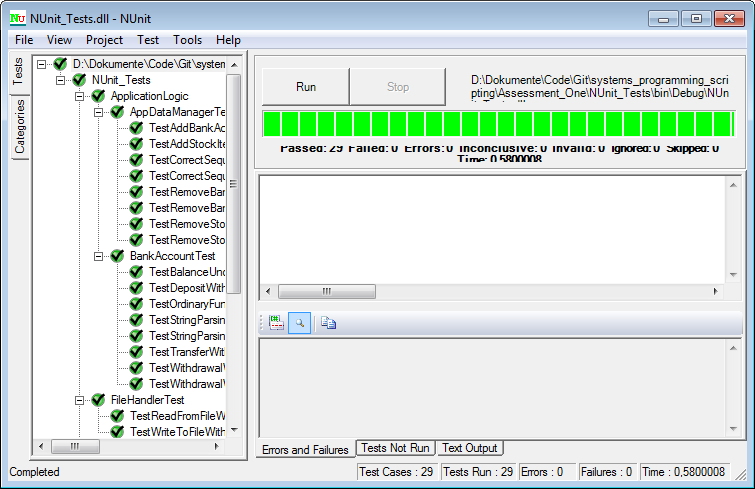
\includegraphics[width=\textwidth]{gfx/nunit.png}
\caption{NUnit test case run}
\label{fig:nunit}
\end{center}
\end{figure}